% =============================================================================================
% SECTION 2 -- METHODS.  Draft 2 -- merge of the former Section 2 (Dataset) and Section 3 (Method).
%
% Two structural faults in the split version are fixed here:
%
%   1. The transfer function -- the substantive contribution -- was 487 words and sat AFTER the
%      816-word regression-model subsection that the deployed route does not even use. The order
%      is now contribution first, auxiliary component second, and the auxiliary subsection is
%      titled for what it actually is ("Supplying a calculation where none exists").
%
%   2. The tier list reported 505 under a definition that only 289 compounds satisfy. 505 is the
%      database's first-principles flag; 289 is the stricter method-string match. Both numbers are
%      correct and are now presented as the refinement they are, with the 214 + 2 remainder.
%
% Statements that appeared twice in the split version are stated once here: the TiNiSn/ZrNiSn row
% imbalance (was in 3.3 and again in 3.5), the fit-objective rule (3.3 and 3.5), and the
% held-out-nulls principle (3.5, 3.6 and twice more in Results).
%
% All labels from the split sections are preserved so existing \ref calls still resolve.
% =============================================================================================

\section{Methods}
\label{sec:method}

We want the \emph{measured} lattice thermal conductivity of a half Heusler, and we obtain it in two
steps: a transfer function that maps a first-principles value onto the experimental scale, and,
only where no calculation exists, a regression model that supplies the first-principles value
itself. The transfer function is the substantive contribution and is described first.
Figure~\ref{fig:method} shows the whole procedure together with the property that organises it.
Measurements and calculations run in separate tracks from the corpus onward and meet only at the
transfer function, so nothing fitted to a calculation is ever scored against another calculation.

\begin{figure}[tb]
  \centering
  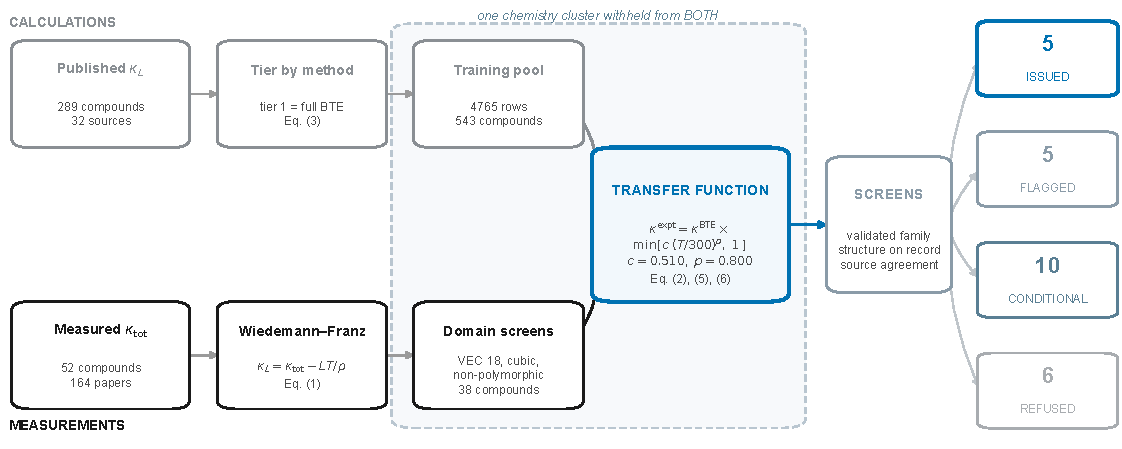
\includegraphics[width=\linewidth]{figures/fig08_method.pdf}
  \caption{\textbf{The method, end to end.} Calculations (upper track) and measurements (lower
  track) are never pooled: they are tiered, filtered and counted separately and meet only at the
  transfer function, which is the sole point at which a calculated quantity is mapped onto an
  experimental one. The dashed region marks what a fold of the validation removes---an entire
  chemistry cluster, withheld from the regression model \emph{and} from the calibration, since
  holding one out but not the other would let the transfer function see the compound it is being
  scored on. Counts are the funnel from \num{289} published calculations and \num{52} measured
  compounds down to the five issued predictions; equation numbers refer to
  Section~\ref{sec:method}.}
  \label{fig:method}
\end{figure}

\subsection{Corpus construction}
\label{sec:dataset}
\label{sec:sources}
\label{sec:composition}

A correction between calculation and experiment can only be fitted where both exist for the same
compound, so the first requirement is a corpus in which the two are separately identifiable. Ours
contains \num{967} distinct compounds, of which \num{742} are half Heuslers, drawn from \num{211}
publications and structure repositories---\num{7823} temperature-resolved values across the
half-Heusler subset---and every value carries its provenance and a statement of how it was
obtained.

Experimental values come from the Starrydata curated transport
database~\cite{katsura2025starrydata}, read at the published snapshot of 1 July
2025~\cite{mato2025starrydata}, from direct extraction of primary publications, and from targeted
recovery of measurements that existed in our own extraction records but had never reached the
training table. The two Starrydata citations are the resource and the dated version actually used,
so the corpus can be regenerated exactly. Starrydata supplies \SI{95}{\percent} of the experimental
rows, and those rows trace to \num{150} distinct primary publications, since it aggregates
digitised transport curves and does not measure anything itself. Seven compounds
(\ce{AlNiSb}, \ce{AlVNi}, \ce{DySbPt}, \ce{LuSbPt}, \ce{TbSbPt}, \ce{VNiSn}, \ce{ZrSbIr}) enter
only through direct extraction, and three of them---the \ce{Sb}--\ce{Pt} series members---validate
a bonding family in which we later issue predictions.

Direct extraction from primary publications was performed by a multimodal large language model
(Google Gemini) reading the full text, tables and figures. The method is
productive but not trustworthy on its own, and one failure mode is worth recording because it is
invisible without an explicit check. A publisher's full-text endpoint may return a metadata stub
carrying only a title and a link, and return it with an HTTP success code; \num{167} such stubs were
stored as though they were articles. Given a title alone the model does not decline. It returns
fluent and specific measurements---instrument models, sample densities, figure numbers, whole
temperature series---that are entirely fabricated. Extraction of \num{45} of those stubs produced
\num{1571} invented measurements, of which \num{524} thermal-conductivity rows reached the export
and accounted for \SI{17.4}{\percent} of it before the defect was found. Two safeguards follow.
Extraction is now gated on the retrieved source exceeding \num{3000} bytes, an order of magnitude
below the smallest genuine article body and above the largest observed stub, so a title-only record
is never sent to the model; and affected rows are flagged in place and excluded downstream rather
than deleted, so the contamination remains auditable. Every surviving value must additionally pass
the physical and provenance gates below, which are enforced in code. No
value enters the corpus on the model's authority alone.

First-principles values were drawn from
AFLOW---transport values from its AAPL module~\cite{plata2017an} and quasi-harmonic estimates from
AGL~\cite{toher2014highthroug}, which the tiering below keeps apart---the Materials
Project~\cite{jain2013commentary}, JARVIS~\cite{choudhary2020the}, OQMD~\cite{kirklin2015the} and
published phonon-transport studies. Crystal structures were taken from the same repositories
together with COD and OPTIMADE-federated sources~\cite{andersen2021optimade}.

Experiments measure total thermal conductivity, so the lattice component must be separated from the
electronic one. We do this by Wiedemann--Franz subtraction,
%
\begin{equation}
  \kappa_L = \kappa_\mathrm{tot} - \frac{L T}{\rho},
  \label{eq:wf}
\end{equation}
%
with the Lorenz number $L$ taken from the single-parabolic-band parameterisation of Kim and
Snyder~\cite{kim2015characteri}, $L = 1.5 + \exp(-|S|/116)$ in units of
\SI{1e-8}{\watt\ohm\per\kelvin\squared} with the Seebeck coefficient $S$ in
\si{\micro\volt\per\kelvin}. \SI{85}{\percent} of the experimental rows are obtained this way; the
remainder are reported as lattice conductivity directly. Equation~\eqref{eq:wf} is a difference of
two measured quantities and is only as trustworthy as the resistivity entering it, so we require
$\rho$ to lie in \SIrange{1e-8}{1e-2}{\ohm\meter}, the range physically available to a dense
intermetallic. Rows carrying $\rho$ of order \SI{10}{\ohm\meter}---six orders of magnitude too
large---drive $LT/\rho$ to zero, so the subtraction removes nothing and the row ships the
\emph{total} conductivity under a lattice label. The failure is silent, and its signature is an
apparent lattice conductivity that \emph{rises} with temperature. \num{136} rows failed this gate,
among them all \num{47} rows of \ce{TiCoSn}.

Figure~\ref{fig:corpus} shows what the corpus contains and, equally, what the field contains. Of
the \num{742} half Heuslers with a thermal-conductivity record of any kind, \num{289} carry a
transport calculation and \num{52} have been measured. The measured set is itself unevenly
evidenced: twenty-seven of the \num{52} rest on a single publication, while five have been measured
by ten or more independent groups. We retain both and carry the distinction forward, so that
agreement with a twenty-times-replicated curve is never presented as equivalent to agreement with a
single digitised figure. Overall, Fig.~\ref{fig:corpus} fixes the two facts the rest of the paper
works from: calculations outnumber measurements by \num{5.6} to one, and the measurements rest on
very uneven evidence.

\begin{figure}[tb]
  \centering
  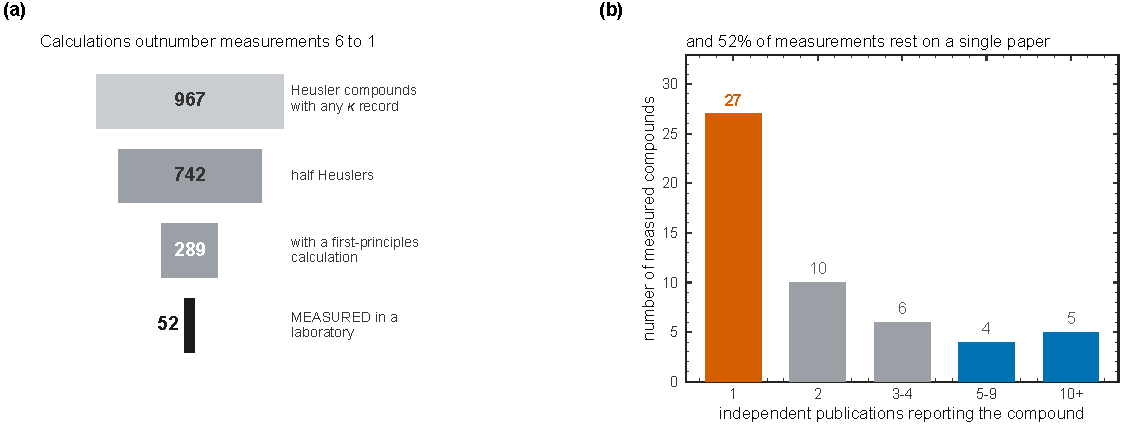
\includegraphics[width=\linewidth]{figures/fig01_corpus.pdf}
  \caption{\textbf{First-principles calculations of half-Heusler lattice thermal conductivity
  outnumber laboratory measurements by \num{5.6} to one.}
  (a) Compounds surviving each stage of corpus construction, drawn to scale. Of \num{967} Heusler
  compounds with a thermal-conductivity record, \num{742} are half Heuslers, \num{289} carry a
  full Boltzmann-transport calculation and \num{52} have been measured.
  (b) Independent publications behind each measured compound. Twenty-seven of \num{52} rest on a
  single source, which sets the evidence tiering used in Section~\ref{sec:results}.}
  \label{fig:corpus}
\end{figure}

\subsection{Method tiering and quality control}
\label{sec:tiering}
\label{sec:gates}

Pooling a measurement with a calculation would destroy the quantity this paper sets out to measure,
so every row carries a \emph{method tier} recording how its value was obtained. Tier~0 is a
laboratory measurement: \num{52} half Heuslers, \num{3482} values, \num{164} publications,
\SIrange{200}{1122}{\kelvin}. Tier~1 is a solution of the phonon Boltzmann transport equation from
third-order force constants. Tier~2 is transport computed on a machine-learned interatomic
potential rather than \emph{ab initio} forces, \num{419} compounds. Tier~3 is a semi-empirical
Slack or Debye--Callaway estimate from elastic and thermodynamic quantities, \num{245} compounds.

For tier~1 the repository flag and the method string disagree. \num{505} half
Heuslers carry a nominally first-principles label, but only \num{289} carry a method string that
positively identifies a transport calculation; \num{214} (\SI{42}{\percent}) carry \emph{only} a
semi-empirical estimate, and two more (\ce{LaSeCl} and \ce{NaSrP}) are labelled merely as an
approximate transport calculation. We assign the tier from the method string and require a positive
match, so that a label we cannot classify counts against us. Throughout this paper tier~1 therefore
means the \num{289}, not the \num{505}.

The two populations are not interchangeable, and the corpus lets us say by how much. For the
\num{93} half Heuslers carrying both kinds of label at a matched temperature, the median
disagreement is a factor of \num{1.38} and \SI{84}{\percent} agree within a factor of two---but the
tail reaches \num{7.2}. The difficulty is dispersion rather than bias: a semi-empirical value is
usually close and occasionally very wrong, and nothing in the value itself indicates which. A
corpus that assigned tiers by repository would average the two and would calibrate a transfer
function partly against values that are themselves fitted estimates.

Five further conditions are enforced in code at the point the corpus is generated, so a rejected
value cannot return when a script is re-run. A compound is admitted as a half Heusler only if a
cubic $C1_b$ record (space group 216) exists in a source that is not a prototype-substitution
database, since prototype decorations record that a structure was \emph{generated}, not that the
phase forms. A compound also recorded in a non-cubic space group is flagged: \ce{MgAgSb} (space
groups 129 and 216) and \ce{DySbPd} (186, 194 and 216) are both dimorphic, and a cubic calculation
cannot be compared to a measurement of a distorted phase without saying so. Half and full Heuslers
are separated by the measured site ratio, not by formula appearance, since a binary in space
group 225 is fluorite, not a Heusler. Values below \SI{200}{\kelvin} are excluded, because the
boundary-free conductivity returned by a transport calculation diverges as $T\to 0$ when Umklapp
scattering freezes out, while the measurement becomes boundary-limited and therefore specific to
the specimen's microstructure; below \SI{200}{\kelvin} the two are not the same quantity. And a
tier-1 row must carry a transport-calculation method string, not a semi-empirical one.

\subsection{The transfer function}
\label{sec:transfer}

A first-principles calculation describes a perfect, infinite crystal, while a laboratory specimen is
a polycrystal with grain boundaries, point defects and finite density, each of which scatters
phonons the calculation allows to propagate freely; for the XNiSn half Heuslers this has been
analysed directly against measurement~\cite{schrade2017the}. The measured conductivity is
accordingly lower, and lower by an amount that grows as the intrinsic phonon mean free path
grows---that is, as temperature falls. We capture this with two parameters,
%
\begin{equation}
  \kappa_L^{\,\mathrm{expt}}(T) \;=\; \kappa_L^{\,\mathrm{BTE}}(T)\;
    \min\!\left[c\left(\frac{T}{300}\right)^{p},\,1\right],
  \label{eq:transfer}
\end{equation}
%
where $c$ sets the room-temperature reduction and $p$ its temperature dependence, and the cap at
unity enforces the physical requirement that extrinsic scattering can only reduce conductivity.
Fitted on the in-domain compounds, $c=\num{0.51}$ and $p=\num{0.80}$. Both are fitted quantities
rather than constants of nature: across leave-one-chemistry-out refits $c$ stays within
\numrange{0.48}{0.51} while $p$ ranges over \numrange{0.80}{1.45}. The suppression at
\SI{300}{\kelvin} is therefore well determined and its temperature dependence is not, and we report
both ranges rather than only the flattering one.

Equation~\eqref{eq:transfer} is not, however, a boundary-scattering model, and the reason is a
bound rather than a preference. A Callaway grey-boundary
treatment~\cite{callaway1959model} with a single boundary length gives a suppression
$S = \Lambda_\mathrm{b}/(\Lambda+\Lambda_\mathrm{b})$ which, with $\Lambda \propto 1/T$, has
logarithmic slope $1-S$ at \SI{300}{\kelvin}---so a boundary model reproducing $S(300)=c$ must have
$p = 1-c$. Generalising to a spectral model, with a per-mode suppression $S_\omega$ and any
distribution of mode conductivities, the slope is
$1 - \langle S^2\rangle_\kappa/\langle S\rangle_\kappa \leq 1-\bar S$ by the Cauchy--Schwarz
inequality. The constraint is therefore not a modelling convenience but a \emph{ceiling}: no
single-boundary-length model, grey or spectral, can produce a slope above $1-c$. At $c=\num{0.51}$
that ceiling is \num{0.49}, and our fitted $p=\num{0.80}$ exceeds it by a factor of \num{1.63}.
Raising the ceiling would require intrinsic mean free paths steeper than
$\Lambda \propto T^{-1.63}$, and the calculations we are correcting do not show that: their own
logarithmic slopes have a median of $-1.00$.

We therefore report the two-parameter form together with the conclusion that follows from it:
\textbf{the correction is not boundary-limited transport}. Its magnitude is of the right order for
grain-boundary scattering in these materials, but its temperature dependence is steeper than that
mechanism alone allows, which implies at least one further temperature-dependent contribution.
Equation~\eqref{eq:transfer} is an empirical transfer function, and we attach no mechanism to its
parameters.

\subsection{What is predicted, and how it is scored}
\label{sec:definitions}

The calculated quantity being calibrated is the phonon Boltzmann-transport conductivity,
%
\begin{equation}
  \kappa_L^{\,\mathrm{BTE}} \;=\; \frac{1}{V}\sum_{\mathbf{q},s}
    C_{\mathbf{q},s}\, v_{g}^{2}(\mathbf{q},s)\, \tau(\mathbf{q},s),
  \label{eq:bte}
\end{equation}
%
the sum over phonon wavevectors $\mathbf{q}$ and branches $s$ of the mode heat capacity, the squared
group velocity and the lifetime. Equation~\eqref{eq:bte} is what every tier-1 source computes and
what Eq.~\eqref{eq:transfer} maps onto experiment; it also fixes what a descriptor must capture to
be useful, since only three quantities enter.

Errors are reported \emph{per compound}, never per row. For compound $i$ with $n_i$ matched
temperatures, and writing $\hat{\kappa}$ for the calibrated prediction and $\kappa$ for the
reference,
%
\begin{equation}
  e_i \;=\; \operatorname*{median}_{j=1\ldots n_i}
    \frac{\bigl|\hat{\kappa}(T_{ij}) - \kappa(T_{ij})\bigr|}{\kappa(T_{ij})},
  \qquad
  r_i \;=\; \operatorname*{median}_{j} \frac{\hat{\kappa}(T_{ij})}{\kappa(T_{ij})},
  \label{eq:err}
\end{equation}
%
and the reported figures are $\operatorname{median}_i e_i$ and the fraction of compounds with
$\tfrac{1}{2} \le r_i \le 2$. The distinction is load-bearing rather than pedantic: \ce{TiNiSn} and
\ce{ZrNiSn} alone contribute \num{753} and \num{646} of the \num{2426} matched rows, so a per-row
median would report those two compounds and call it a method. For the same reason the calibration
is fitted to the quantity that is reported,
%
\begin{equation}
  (c, p) \;=\; \operatorname*{arg\,min}_{c,\,p}\;
    \operatorname*{median}_{i \in \mathcal{T}} e_i(c, p),
  \label{eq:fit}
\end{equation}
%
over the training compounds $\mathcal{T}$ of a fold. Fitting one objective and reporting another has
cost this project a spurious \num{9} percentage points once already.

\subsection{Domain of applicability}
\label{sec:domain}

A transfer function for \emph{lattice} thermal conductivity is meaningful only where lattice
conduction is the dominant channel, so we state in advance where the method applies. First, the
compound must have eighteen valence electrons. Half Heuslers are semiconducting at the closed-shell
counts, of which $\mathrm{VEC}=18$ is the one relevant to transition-metal
members~\cite{graf2011simple,anand2018a}; away from such a count the compound is metallic, a large
electronic term must be removed from every measurement, and $\kappa_L$ no longer governs transport.
Main-group members such as \ce{LiAlSi} are semiconducting at $\mathrm{VEC}=8$, and we restrict to
18 because that is where the corpus has support, not because 8 is metallic. Electrons are counted
as the group number for groups 1--12 and group$-10$ for the $p$ block; \ce{Yb} is divalent in many
antimonides, which would move \ce{YbNiSb} out of the domain, and we flag it rather than rely on the
count. Second, the structure must be cubic $C1_b$ and not polymorphic, since the calculation being
calibrated is for the cubic phase. Third, no constituent may be an actinide or otherwise
radioactive, for which the corpus contains no training example.

Of the \num{51} half Heuslers with both a measurement and a calculation, \num{38} satisfy these
conditions. These three screens are applied identically to the validation set and to every issued
prediction, and none was chosen after inspecting the results. Section~\ref{sec:screening} adds two
further conditions before a prediction is \emph{issued}---that the bonding family already contains
validated members, and that the value falls inside the range that family has been measured in---and
those two are properties of the prediction pipeline rather than of the domain. They are stated, and
tested, where they are used.

Several sub-populations of these \num{38} recur in what follows, and because the accuracy figures
quoted for them are not comparable across populations, Table~\ref{tab:populations} defines each
once.

\begin{table}[tb]
  \centering
  \caption{The compound populations used in this paper. Every accuracy figure is quoted over one of
  these, and figures over different rows are not directly comparable---a point that matters most
  when the method is set against the family baseline, which is defined only on the \num{31}.}
  \label{tab:populations}
  \begin{tabular}{clp{0.56\linewidth}}
    \toprule
    $n$ & name & definition \\
    \midrule
    \num{742} & half-Heusler corpus & any thermal-conductivity record of any kind \\
    \num{289} & calculated & carries a full Boltzmann-transport calculation \\
    \num{52}  & measured & has ever been measured in a laboratory \\
    \midrule
    \num{51}  & matched & has both a measurement and a calculated value \\
    \num{38}  & \textbf{in-domain} & the \num{51} after the three domain screens; \textbf{the blind
                test set, and the population behind every headline figure} \\
    \num{13}  & excluded & the remainder of the \num{51}, scored separately in
                Section~\ref{sec:failure} \\
    \midrule
    \num{34}  & published-matched & of the \num{38}, those also carrying a temperature-matched
                \emph{published} transport value; the offset of Section~\ref{sec:offset} and the
                deployed-route scores of Section~\ref{sec:deployed} \\
    \num{31}  & family-covered & of the \num{38}, those whose $(\mathrm{Y},\mathrm{Z})$ family holds
                at least two other measured members; the only population on which the family
                baseline is defined \\
    \num{28}  & curve-resolved & of the \num{38}, those with at least five measured temperatures
                spanning \SI{300}{\kelvin} \\
    \num{21}  & semi-empirically covered & of the \num{38}, those carrying a published Slack or
                Debye--Callaway estimate \\
    \bottomrule
  \end{tabular}
\end{table}

\subsection{Supplying a calculation where none exists}
\label{sec:model}

The transfer function needs a calculation to correct, and for a candidate compound there may not be
one. We therefore train gradient-boosted decision trees
(CatBoost~\cite{prokhorenkova2017catboost}) on \num{45} inputs: \num{42} descriptors of composition
and the $C1_b$ geometry---elemental masses, radii, electronegativities and their contrasts across
the three sites, volume per atom, density, and nearest-neighbour bond lengths with their
spread---together with three encodings of temperature ($T$, $1000/T$ and $\log_{10}T$). This model
is a fallback, not the deployed route: where a transport calculation already exists, calibrating it
gives \SI{29.7}{\percent} median error against \SI{43.0}{\percent} for the model on the same task,
and the model is not used.

Two details of the descriptor set matter. Lattice parameters must be reduced to a single convention
before use, because four of our structure sources publish the primitive face-centred edge and one
the conventional cell, related by $a_\mathrm{conv} = \sqrt{2}\,a_\mathrm{prim}$; mixing them
injects a \SI{41}{\percent} error into every length descriptor and \SI{183}{\percent} into
volume-derived ones. The lattice parameter is therefore never emitted as a descriptor in either
convention, and volume per atom carries the same physics while being convention-independent.
Bond-length descriptors in turn require explicit atomic coordinates, and where a record lacked them
we supply the ideal $C1_b$ positions instead of letting the features fall through as missing---six
compounds were previously scored on \num{41} of \num{45} descriptors for want of this.

The training pool is \num{4921} compound--temperature rows over \num{686} compounds spanning
\SIrange{200}{1200}{\kelvin}. \num{4765} of those rows carry a full Boltzmann-transport
calculation; a further \num{156} carry only a semi-empirical estimate and enter at a reduced sample
weight of \num{0.3}, because they cover chemistries for which no transport calculation exists
anywhere. Those rows retain tier~3, enter only as down-weighted training signal, are never used as
a reference value and carry no reported statistic, so admitting them bends no tiering rule. The
pool is likewise not restricted to half Heuslers, since the descriptors are structural and
compositional rather than prototype-specific; held-out scoring is always on half Heuslers alone.

Whether the choice of regressor matters is a question we tested. Four model
families---gradient-boosted trees in two implementations, kernel ridge regression and a Gaussian
process---were trained on identical rows and descriptors under the same grouped cross-validation,
on the \num{4765}-row transport part of the pool alone. They do not agree on a winner: CatBoost has
the best coefficient of determination on $\log_{10}\kappa_L$ (\num{0.889} against
\numrange{0.760}{0.872}) while LightGBM has the lower median error (\SI{22.0}{\percent} against
\SI{25.7}{\percent}). That disagreement concerns fit to \emph{calculated} labels, so we repeated
the entire blind test with LightGBM in place of CatBoost, under the same folds, holdout, nested
calibration and scoring. It gives \SI{37.1}{\percent} median error and \SI{78.9}{\percent} within a
factor of two against \SI{31.0}{\percent} and \SI{86.8}{\percent} for CatBoost on the same \num{38}
compounds; LightGBM is better on \num{17} of them, and a paired signed-rank test does not separate
the two ($p = \num{0.45}$). The advantage LightGBM holds on calculated labels does not survive
calibration to experiment, and the gap between the two is smaller than the spread the headline
shows across model seeds. We retain CatBoost and record that the choice is not load-bearing.
Figure~\ref{fig:model} shows both results: which regressor was chosen, and what the retained model
rests on.

\begin{figure}[tb]
  \centering
  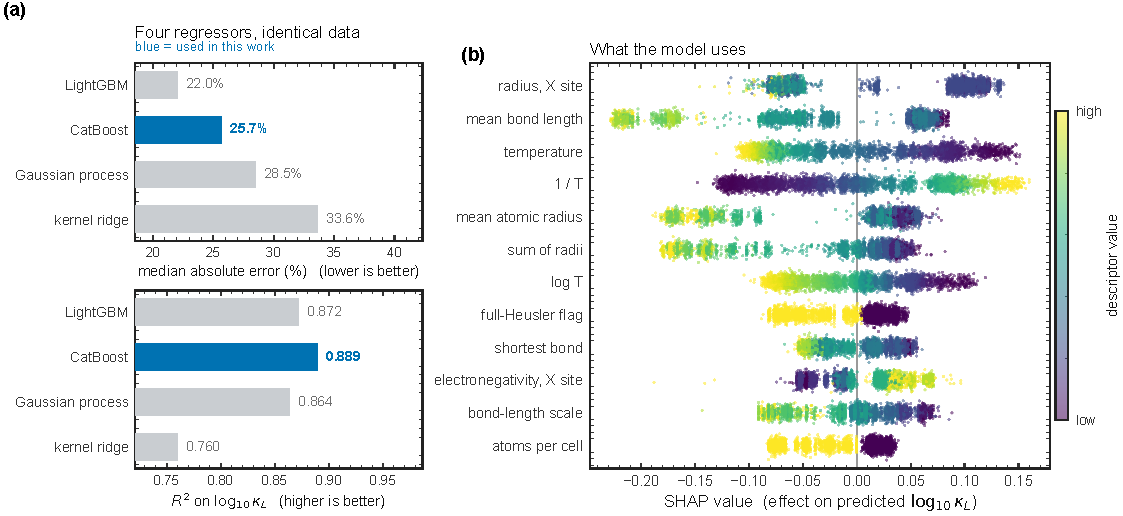
\includegraphics[width=\linewidth]{figures/fig07_model.pdf}
  \caption{\textbf{The regression model: which one, and what it uses.} (a)~Four regressors on
  identical rows and descriptors under grouped cross-validation with whole chemistries held out.
  The two metrics disagree---CatBoost leads on $R^2$, LightGBM on median error---so the blue bar
  marks the model retained, not a winner. (b)~SHAP decomposition of the retained model: for every
  row, how far each descriptor moved the predicted $\log_{10}\kappa_L$, coloured by that
  descriptor's own value. The signs are those thermal transport requires---larger radii, longer
  bonds, more atoms per cell and higher temperature all push $\kappa_L$ down---so the fit rests on
  phonon physics rather than on an artefact of the corpus.}
  \label{fig:model}
\end{figure}

\subsection{Validation, null baselines and prediction intervals}
\label{sec:validation}
\label{sec:nulls}
\label{sec:intervals}

Every figure we report is obtained with the target compound's \emph{entire chemistry} withheld from
training. Compounds are clustered by their most electropositive site and a whole cluster is removed
at once. Compounds sharing the held-out compound's $(\mathrm{Y},\mathrm{Z})$ bonding family but
built on a different X site do remain in training---\num{33} of the \num{38} in-domain compounds
have at least one such relative---so the test measures accuracy for a new X-site substitution
within a known bonding family. It is nonetheless a harder test than removing single compounds,
under which near-duplicates of the target survive in training.

Three precautions make that holdout mean what it says. Any threshold or model choice is made on one
half of the chemistry clusters and evaluated on the other, since selecting on the same data one
reports inflates the result by \SIrange{7.7}{10.3}{pp} depending on the protocol, which we measure
rather than assume. Every reported figure is the median over five model seeds and is quoted with
its across-seed range: the median error moves from \SI{31.0}{\percent} to \SI{40.0}{\percent}
across seeds, so a single-seed figure reports the seed as much as the method, whereas the
within-$2\times$ fraction (\SIrange{81.6}{86.8}{\percent}) and the rank correlation
(\numrange{0.618}{0.675}) are stable, which is why we lean on them. And the two calibration
parameters are themselves refitted with the scored compound's cluster removed; fitting them once on
all \num{38} compounds and scoring the same \num{38} would report \SI{29.7}{\percent} rather than
\SI{31.0}{\percent}.

A method that predicts $\kappa_L$ must beat predictors that use no compound-specific information at
all. We use two: a constant equal to the median measured conductivity of the training compounds,
and a power law $A(T/300)^{q}$ fitted to them. Both are fitted with the same chemistry held out as
the calibration, since a null given less information than the method is not a test of anything.

Intervals are conformal, taken from the out-of-fold residual distribution in logarithmic space
because the error is multiplicative. For a nominal level $\alpha$, over the $m$ held-out compounds
of the declared domain,
%
\begin{equation}
  \delta_\alpha \;=\; \Bigl\{\, \bigl|\log_{10} r_i \bigr| \,\Bigr\}_{(k)},
  \qquad k = \bigl\lceil (m+1)\,\alpha \bigr\rceil,
  \label{eq:conformal}
\end{equation}
%
the $k$-th order statistic of the absolute log-residuals, giving the multiplicative half-width
$10^{\delta_\alpha}$. The $(m+1)$ and the ceiling are both required for finite-sample validity;
the empirical $\alpha$-quantile under-covers at these sample sizes. Coverage is evaluated
leave-one-chemistry-out---the band applied to a held-out cluster is built only from the residuals
of the other clusters---and tracks nominal closely: \SI{50}{\percent} nominal gives
\SI{50.0}{\percent}, \SI{80}{\percent} gives \SI{81.6}{\percent} and \SI{90}{\percent} gives
\SI{92.1}{\percent}, with multiplicative half-widths \num{1.31}, \num{1.92} and \num{2.24}. A
stated interval is therefore a measured frequency rather than an assumption, though on \num{38}
compounds these frequencies carry a binomial uncertainty of roughly \SI{8}{pp} and should be read
as consistent with nominal rather than as precise.
